% Appendix A

\chapter{Évitement d'obstacle} % Main appendix title

\label{AppendixA} % For referencing this appendix elsewhere, use \ref{AppendixA}

%\section{titre de la section}

Plusieurs cas de figure existent selon la position des obstacles par rapport à celle du robot, pour cela nous avons étudié toutes les possibilités pour garantir le bon fonctionnement de notre approche dans tous les environnements.\\

La figure \ref{choix_annexe} représente deux cas de figure se produisant souvent dans des environnements complexes.
Lorsque aucune trajectoire admissible n'est trouvée dans le champ de vision initial du robot (90$\textordmasculine$), on l'élargit aux zones adjacentes de 90$\textordmasculine$ allant ainsi à un champ de vision qui équivaut les 270 $\textordmasculine$. Ceci simulera une rotation du robot sur lui même (voir schéma de droite).

Si aucune trajectoire admissible n'est trouvée par le robot , une nouvelle position destination est demandée.
\\

Aussi dans le cas ou la position destination est alignée sur un des deux axes avec la position actuelle du robot, (c'est-à-dire qu'ils possèdent la même abscisse ou même ordonnée) notre robot aura une vue sur les 180$\textordmasculine$ dont la droite (position du robot - position destination) est commune (schéma de gauche).
\noindent
\begin{center}	  
	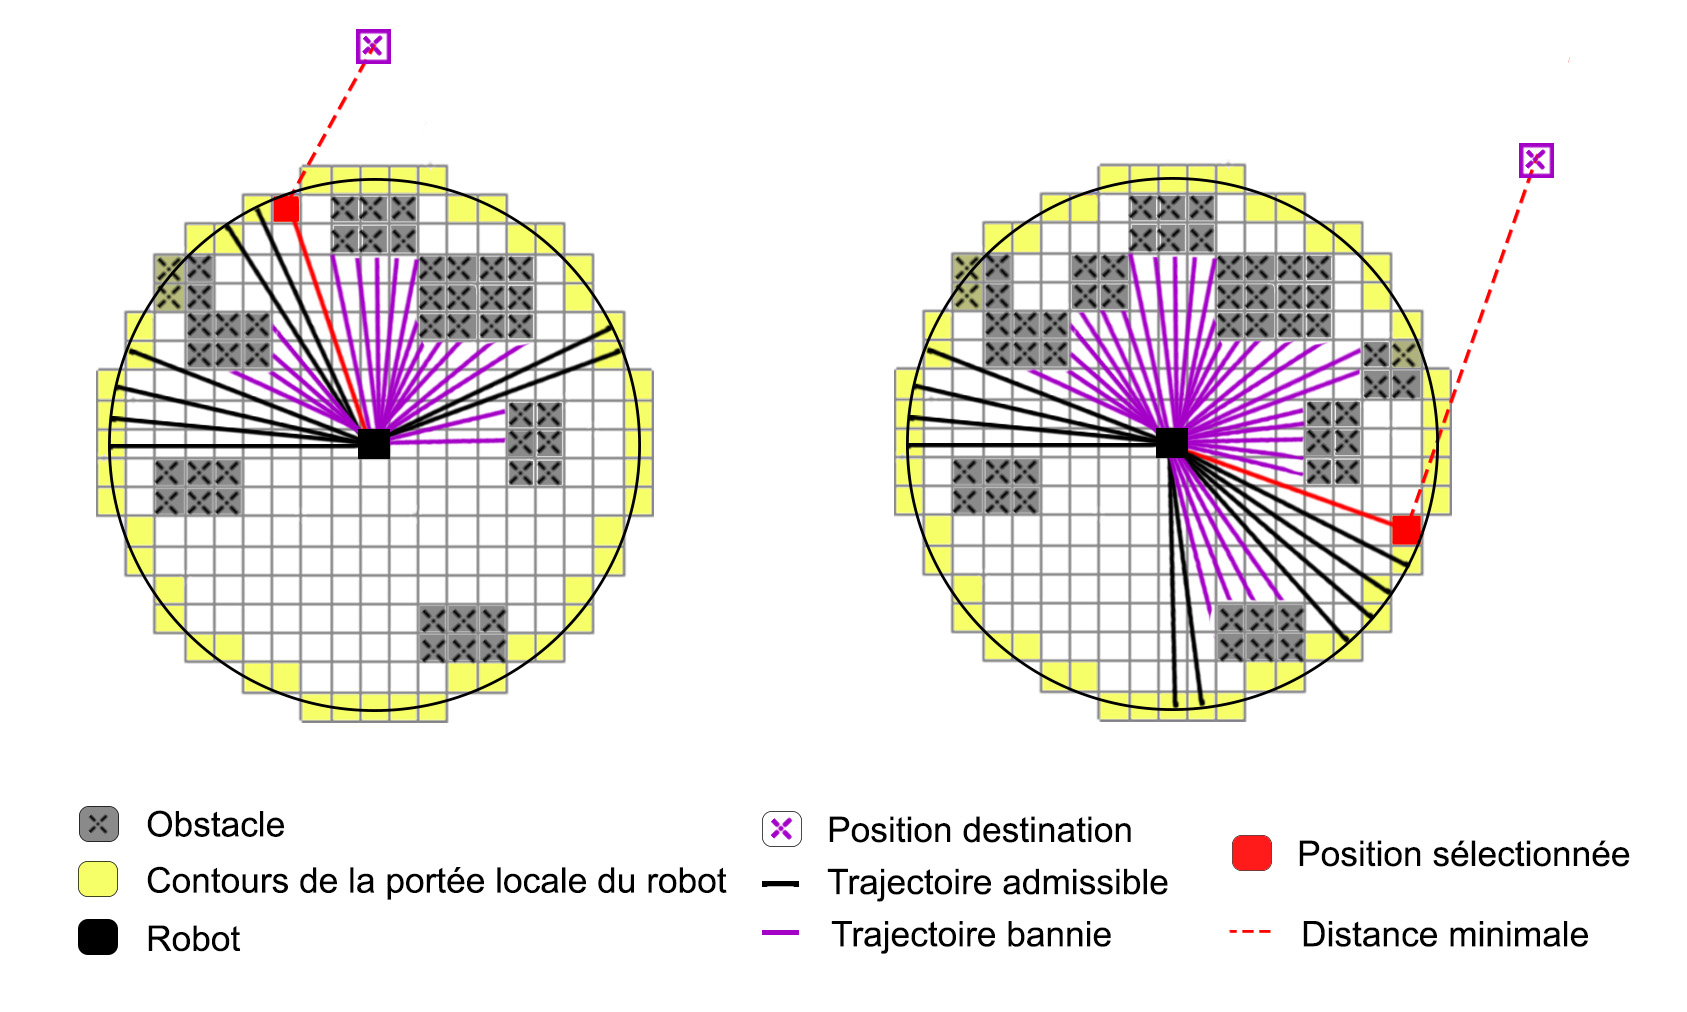
\includegraphics[width=1.1\textwidth]{choix_annexe.jpg}%
	\vspace{-0.1 cm}
	\captionof{figure}{Choix de la trajectoire à suivre par le robot dans des situations complexes.}\label{choix_annexe}%
\end{center}

